\documentclass[12pt,a4paper,oneside,openany]{book}
\setcounter{secnumdepth}{3}
\usepackage{xcolor}
\usepackage{minted}
\usepackage[utf8]{inputenc}
\usepackage{tikz}
\usepackage{caption}
\usepackage{gensymb}
\usepackage{lmodern}
\usepackage{multirow}
\usepackage{booktabs}
\usepackage{array}
\usepackage{adjustbox}
\usepackage{upquote}
\usepackage{amsmath}
\usepackage{listings}
\usepackage{titlesec}
\usepackage[hidelinks]{hyperref}
\usepackage{fancyhdr}
\usepackage{graphicx}
\usetikzlibrary{mindmap,shadows, shapes, arrows, positioning}

\begin{document}
\begin{titlepage}
\newcommand{\HRule}{\rule{\linewidth}{0.1mm}} 
\center % Center everything on the page


\HRule \\[0.4cm]
{ \huge \bfseries Farming App - Built with the Ionic 3 Framework}\\[0.1cm] % Title of your Homework/assignment
\HRule \\[1.5cm]

 \begin{center}
    {\Large
      \textbf {Gary Mannion}
    }\\
    \vspace{0.2cm}
    {\Large
     \textbf {Derrick Conway}
    }
  \end{center}
  
  \begin{center}
      B.Sc.(Hons) in Software Development
  \end{center}
  
  \vfill

{\large \today}\\[.75cm] % Date, change the \today to a set date if you want to be precise

\begin{center}
    {\large
    \textbf {Final Year Project} \\[0.1cm]
    }
  \textbf {Advised by: Patrick Mannion} \\[0.1cm]
      Department of Computer Science and Applied Physics\\
      Galway-Mayo Institute of Technology (GMIT)    
\end{center}
  
\begin{center}

\includegraphics[width=1.0\textwidth]{Images/gmitlogo.jpg} \\

\end{center}
\end{titlepage}

\newpage
\tableofcontents

\newpage
\listoffigures
\renewcommand{\thefigure}{\arabic{chapter}.\arabic{figure}}


\newpage

\chapter*{Abstract}
For our final year project, we were looking to create an industry stander application that would help farmers in day to day life. There has been a lot of talk in recent weeks about the escalating fodder crisis and the negative impact it is having on farmers and their livestock. For months, farmers have faced difficult farming conditions due to persistent cold and wet weather. Farmers usually purchase enough fodder, dried hay or feed given to cattle and livestock, to last until the spring when the grass begins to grow, and animals can begin to eat that instead. As a team we want to design a free web application where the user can enter data and store it, do out calculations for the fodder months. There is also AI section for keeping track of the herd in the calving months, tagging section for keeping track of new born animals, section for keeping track of the medicine used on the herd throughout the year. We have created this application with a client and server pulling data from databases. We created a three-tier application, using Mongo Db and Fire-base as our Data Tier, NodeJS for our Logic Tier and Ionic 3 for our Presentation Tier.
Adding specific features such as, adding Al, Tagging, Feed, Madison and creating a message board for farmers to group together and find solution's to problems there are encountering. it was our objectives by gearing our app specifically for farmers. \\

\noindent \textbf{Authors:}

\begin{itemize}
    \item \textbf {Derrick Conway}
    \item \textbf {Gary Mannion}
\end{itemize}


\chapter*{\centering Acknowledgements}
{\large
\noindent We would like to acknowledge our project supervisor Patrick Mannion for his help and supervision during the creation of this application.\\

\noindent We would also like to thank John Healy, Head Lecturer of the Applied Project and Minor Dissertation module. 
}
\chapter{Introduction}
When choosing our project we wanted to pick something that was relevant to current everyday life. We wanted a project that also highlighted our existing skills and allowed us to learn new skills and develop as part of a team. With this criteria in mind we started brain storming ideas for our project.  

We eventually decided on a App called herd list, herd list would be a farming fodder app. We recognized the current fodder crisis throughout Ireland and thought it would benefit farmers and farmers alike to have a specific fodder app for the farming population.
Currently farmers in Ireland can find themselves in difficult situations for up to 1 or 2 months before finding proper fodder for animals.
This is quiet common for farmers and with our app they would only be able for to calculate fodder for the winter and spring months and keep track of tagging, medicine, AI.

Having a fodder app as our starting point we started to research other apps and websites in the farming category. The main one we focused on was the Heard Watch. Heard Watch would be the most popular farming app in Ireland and it provided us with a great deal of insight on what our app would need to have and also on what heard watch lacks for the farming market.

We wanted a app that had essentially the same functionality as Heard Watch but which was geared more towards the stress points of farming We did this by focusing on what stresses farmers the most, We also created a forum for farmers to get in touch with one another, to either get information from one another or to give information, These would compliment the normal functionality of a accommodation app such as, publish ads (either fodder or rent land), search lists, view ads or messages and land for rent and edit and delete your personal ads. This would also require log in and registration functionality.  

After deliberating over the objective of our application, we then turned to what technology we would use. We wanted to use a array of technologies to show our capabilities but also gain more knowledge and become better programmers over all. We settled on a 3 tier structure containing a Ionic 3 presentation tier (front end), NodeJS logic tier (middle-ware)  and MongoDB/CouchDB/fire-base Authentication data tier (back end).

From what we hoped to achieve from creating this app was the knowledge of new technology, personal growth through team building and of course to produce something of substance and something we could be proud of.

\chapter{Context}

The general context of our application revolves around farmers having a platform which is geared towards tracking fodder, and there heard. farmers will be able to calculate amounts of fodder for the winter months and use the app to keep track of the tagging of new born animals, track medicines for animals throughout the year, and store AI information to which heard animal are in calf and how far alone they are gone and when they are due.


\begin{itemize}
	  \item Feed
	  \item AI
	  \item Medicine 
	  \item Tagging
	\end{itemize}


\section{Objectives} \label{objectives}
The main objective of our application is to help farmers who may be struggling with the current fodder crisis in Ireland. We also wanted to make it easier for farmers and farmers alike, who are finding it difficult to keep track fodder, AI, Medicine and Tagging. The following is a list of the main pages in our application along with the objectives for each page. 

\begin{enumerate}
    \item \textbf{Login/Register Page} Our application has a login and a register page. The register page allows the user to securely register with our application while the login page allows the user to securely login to our application. Once logged in, the user has access to extra features not accessible to unregistered users.
    
    \item \textbf{Forgot-Password Page}
    The objective of the forgot-password page is to allow a user who has forgotten their password to enter their email address. They will then receive an email containing a link which will allow them to create a new password.

    \item \textbf{Home Page} 
    The objective of the homepage is that it is a base of navigation for the application. The homepage will also display if a user is logged in or not.
    
    \item \textbf{Feed} 
    The objective of this feed page is to display is to calculate out how much feed you need for the winter months by entering the number of animals on the farm and calculate out how much is needed.
    
    \item \textbf{Tagging} 
    The objective of this tagging page is to keep track of the heard animals calving by inputting the details of birth,gender and breed of the animal. This will allow the user to keep track in an easy way of filling in form details at there own personal time..
    
     \item \textbf{AI}
    The objective of this AI page is to keep track of witch hear animals are in calf and how far gone they are and witch are not in calf this will allow the user to keep track of heard and when they are to calf buy filling in form details as it is being read out.
     
     \item \textbf{Medicine}
     The objective of this medicine page is to keep track of all the animals medicine that have been taken, show when it was taken, how much was taken. This will allow the user to keep track of heard medicine buy filling in form details.
     
     \item \textbf{Scanner}
     The scanner would be used for a user to scan a medicine bottle and specific information would be returned about that specific bottle.
     
    \item \textbf{Message Board} 
    The objective of the message board is to have a place where farmers can communicate with each other, helping themselves and other farmers with problems and place ads for stock.
    
    \item \textbf{My Ads Page}
    The objective of the Ad’s page is to allow a user to view a list of their published ads. In here they can delete these ads or they have the option to edit their published ads.
\end{enumerate}

\section{Project Links}

\paragraph{Link to Repository}
\begin{itemize}
\item \href{https://github.com/Gazza1996/Final-Year-Project-Applied-Diss}{https://github.com/Gazza1996/Final-Year-Project-Applied-Diss} 
\end{itemize}

\section{Chapters Review}
This paper is broken down into different chapters, ranging from planning, design and development. The following sub-sections give a brief overview of each chapter in this paper.

\subsection{Methodology}
In this Chapter we discuss some of the methodologies we used during the various stages of creating the farming app. In this section we discuss Agile, version control, testing and sprints.

\subsection{Technology Review}
In the Technology Review chapter we review the various technologies we used in our project. We review back and front end technologies, development tools and version control.

\subsection{System Design}
In this chapter we give a detailed explanation of the overall system
architecture and design of farmers app. We explain why we chose these specific technologies and how we implemented them into our system design.


\subsection{System Evaluation}
In this chapter we evaluate our system in the areas of Robustness, Testing, Results Versus Objectives and Limitations.


\subsection{Conclusion}
In the conclusion we summaries our project against our goals and objectives. We review our application from the various stages and speak about possible future development.

\chapter{Methodology}

In this chapter we discuss the methodologies used in our project. A methodology is just a way to plan and control the development process of a piece of software. There are various methodologies to choose from including Extreme Programming, Rapid Application Development or Waterfall but for this project we use Agile as our main methodology.


\section{Agile Development}
During the life cycle of our project we attempted to use an Agile like approach to the research, design and implementation stages of the project. In the initial stages of the project we discussed various methodologies we could use, for example Waterfall but we decided on Agile because of waterfalls lack of flexibility. Agile offers continual improvement, flexibility and incremental delivery of the software.  \\

\noindent During the research and development process of our project we used a Scrum like approach. Scrum is an Agile method in which a development cycle is carried out in what are known as sprints. Section 3.4 and 3.5 contains more information on each sprint of the research and development phase of the project. \\

\noindent Throughout the life cycle of the project we held weekly meetings. In these meetings we would plan and discuss the features of our application. Before each sprint of our project, we used these meetings to plan our sprint cycle. Results from these meetings were then added as to-dos and added to a Git-Hub projects page. Git-Hub projects board help us prioritize and organize our work load. We found this to be an especially useful tool. Once an issue was created it was added into the To-do phase. Then, when we started working on a problem it got added to in-progress, then finally into the completed section once the task was done. A snapshot of our Git-Hub Projects page can be found in Figure !!NEED TO INSERT IMAGE OF TODO LIST!!\\

% insert image from projects

\noindent We also had weekly contact with our project supervisor. Our supervisor was instrumental in advising us on our progress and helping us with issues with the project.

\section{Version Control}
Throughout the life cycle of our project we used GitHub. GitHub is a hosting service for version control. We created a GitHub repository, adding all the members of the team to work as collaborators. We found GitHub to be an extremely useful tool in the research and development of Farmers app. Even though we primarily used GitHub to manage source code, we also took advantage of some collaboration features that GitHub offers. We used wikis to track what we learned in the research stages of our project. A wiki is a website where multiple users can modify content directly from their browser. We used GitHub’s task management tool when a task was set and then used this tool to track that tasks progress.  We found this tool particularly useful as it helped break down the workload into small manageable tasks.

\noindent As a team, working with source code on GitHub proved to be its most valuable feature. Git-Hub allows all members of the team to see all the commits made to the repository. We can see every update, previewing every change that was made and even rolling back a commit if necessary.

\section{Testing}
For our application, We needed to make a decision on how we would test the application as we did not choose to use a framework (i.e. J-unit) to test our application, we did however decide to use both white and black box testing.

\subsection{White Box Testing}
White box testing is a way of testing software where the tester can see the internal workings of the software. White box testers have full knowledge of the internal makeup of the software and are usually software developers themselves. In our application, to white box test, one team member would write a feature (e.g. login) and then another team member would test that functionality. That team member would present input, follow the path through the code and then examine the output. A diagram of white box testing can be found in Fig \ref{white_box} \\
\begin{figure}[ht]
\renewcommand\thefigure{3.1}
\centering
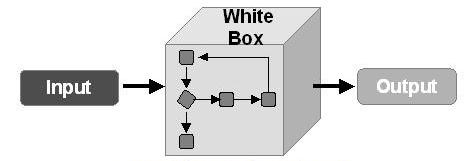
\includegraphics[width=8cm, height=3cm]{Images/whitebox.jpg},
\caption{White Box Testing}
\label{white_box}
\end{figure}


\subsection{Black Box Testing}
Black box testing is a way of testing a piece of software without knowing the internal functionality of the software being tested. A black box tester has no knowledge of the internal design, structure or implementation of the software and are often not programmers themselves. In our application, to black box test, we would ask friends to use our application e.g. asking them to login to the application and to maneuver through the application and then reporting their experience. With this type of testing, the tester is trying to break your application looking for faults. We found this type of testing especially useful as it gave us an insight into the way a user would use our application, something we previously would not have thought of when developing this farming application. A diagram of black box testing can be found in Fig \ref{black_box} 

\begin{figure}[ht]
\renewcommand\thefigure{3.2}
\centering
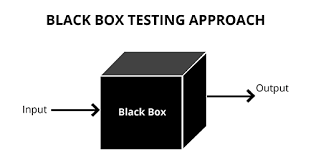
\includegraphics[width=8cm, height=3cm]{Images/blackbox.png},
\caption{Black Box Testing}
\label{black_box}
\end{figure} 

\noindent The following two sections contain information about the various sprints we undertook in the research. \\


\section{Sprints} \label{reseacrh_sprints}
In this section we shall be discussing the sprites, Each of the sprints we completed during the research of our project gave us the opportunity to learn as a team and adapt to the various needs of the project. Each sprint represents a vital aspect of the application, i.e., creating three tier architecture, accessing native phone capabilities through Cordova and learning how to integrate all these features together. We prioritized the research sprints in the order as follows.

\subsection{Sprint 1 Review King}
This was our first sprint and it was worked on by all members in our team. we researched a simple app in which it explains the process of building a simple review app using three tier technology. On the front end a user can write a small review and then add a score. That information is then sent to a node server which stores the information in a MongoDB database. We felt it was very important that all members understood the process involved in connecting these three layers together so we all worked on this sprint together.   

\subsection{Sprint 2 "cloudo"}
For our research in this sprint we look at using pouch DB and couch DB in our app in one of our pages just to offer us another Database choice if we encountered any problems down the line. We researched a simple app called "cloudo" which we both worked on and built step-by-step in order to understand how these Databases would work in our ionic project. We simply would just import Pouch DB into our project, get Pouch DB to call our Couch DB database using a remote link on our local-host, create a database giving it a name 'cloudo'. once this is done we would be able to write to our Database from a page and update/delete if need be.

\subsection{Sprint 3 Login/Register}
In this sprint, implemented by Patrick, a small mobile application was developed where login and registration with Fire-base was implemented. We are using Fire-base in our farming application to securely authenticate our users with email and password registration and login. 

\section{Development Sprints}\label{development_sprints}

\subsection{Sprint 1 Create Pages}
From the result of team meetings, we had decided on the number of pages our application would require. In the first development sprint, we created all the pages that we would need for our application, And added a few extra features to the application if we had time to do these extra features example, scanner and camera war the extra features. The sprint was completed by the members of this project and this formed the base skeleton of the farming application.

\subsection{Sprint 2 Menu Navigation}
The next step was to implement a menu into our app connecting all the pages together. The result of this sprint was so that each page could now be navigated to, by either the main menu or by a button on a page. This sprint was completed by the members of the project.

\subsection{Sprint 3 Login/Registration}
For this sprint it was now time to implement the registration and login functionality to the farming application. This was successfully done by a member of the project that implemented this sprint as he had previous knowledge of implementing this functionality with Fire-base from a previously completed research sprint.

\subsection{Sprint 4 Implementing the Back End}
In this sprint we implement our NodeJS server running on one of our AWS instances. This sprint was completed by members of the project and in it we set up our API routes along with MongoDB to store text data in our database. The text data being stored would be the data from a created listing i.e. breed, tag number, Date of birth etc...

\subsection{Sprint 5 Feed Calculator}
In this sprite we worked on the how we would use the feed page, we decided to use it as a calculator to calculate out the amount of feed witch would be required by the amount of herd animals on the farm and working out the calculations for the pit and bales that will be required for the winter months ahead. We first implemented the functionality on the front end. Allowing the user to enter the amount needed for the future months, and also show the amount of feed the farmer currently has.

\subsection{Sprint 6 Tagging}
In this sprite we worked on the how we would use the tagging page, we decided to use it as a way of keeping note of the heard animals calving and if there was any complications. We first implemented the functionality on the front end allowing the user to input data of the animal and storing it, the features of this page are to input the animal tag number, breed, date of birth and if there was any complication on the animal giving birth. 

\subsection{Sprint 7 Medicine}
In this sprite we worked on the how we would use the medicine page, we decided to use it as a way of keeping track of the heard animals that have received medicine and note why they needed the medicine and how much was giving and the dates it was giving to the animal, also note if there was any complications. We first implemented the functionality on the front end allowing the user to input data of the animal and storing it,

\subsection{Sprint 8 AI}
In this sprite we worked on the how we would use the AI page, we decided to use it as a way of keeping track of the heard animals that are in calf, We first implemented the functionality on the front end allowing the user to input data of the animal and storing it, the information would be how far alone they war, and track with one are not in calf as of yet. so the farmer can track how many to expect for the winter and spring months.



\subsection{Sprint 9 Message Board }
The next task, implemented by the team, was the Message board. The result of this sprint was the creation of a forum in which users can communicate with each other by creating and posting messages. we first set up the back-end to store these messages in MongoDB database and then displays the stored messages to the user. Message output includes the users name, message and date created.

\subsection{Sprint 10 Camera}
This sprint was worked on by all members of our team because taking and storing images is one of the prominent features of farm application. We first implemented the functionality on the front end. This allows a user to take a photo using the camera on their device or by selecting a photo from their devices internal storage. We then implemented our back-end API to store those images mapping each image/s with its unique ad id.

\subsection{Sprint 11 Scanner}
This sprint was worked on by all members of our team as we had no experience in the scanner side of it, the scanner is to scan the ear tag of the animal and show the information of the animal. this was unsuccessful as there war complications. We could scan the tag but needed a scanner to read the information from the tag, cause of this we could not get our hands on one as there war expensive and not many had them.

\subsection{Sprint 12 Search}
One of the last features of our application is the search functionality. Implemented by team members, user can narrow down the tag number information in the tagging page, medicine page and AI page. We first implemented the functionality on the front end allowing the user to input data of the animal and searching it.


%\subsection{Sprint 13 Validation}
%In this sprint Patrick and Gerard implemented form validation on the register, login, message board and create ad pages. For the matching passwords validation, we created a custom function which checks that the passwords are the same. For all other form validation, we use Angular directives to check that correct input is entered and that all fields are complete before the from can be processed. 

\chapter{Technology Review}
In this section, we will cover the overall design and architecture of our Application. We will do this through code snippets and visual aids to help you get an understanding of the Application design. The System Design chapter will be broken up into three parts. Data Tier represented by our Databases MongoDB and Fire-base, Logic Tier represented by NodeJS servers, Presentation Tier which will be represented by Ionic 3 App and our deployment of our app. 

\section{Data Tier}
The data tier represents the overall stored data and gives the ability to store, access, update and delete certain data. For our application we have two databases. One database is used to store our user accounts and the other is used to store our users information and messages.

\subsection{Fire-base Authentication}
We chose Fire-base to handle our user accounts as it was established in the ionic community for being a good database for login and registration functionality. The Fire-base Authentication SDK provides methods for creating and managing users who use email and password to log on to the system. Fire-base uses tokens to allow users to login/logout and to register to an Application. The fire-base documentation states that the listener receives notifications in the following: 
\begin{enumerate}
    \item When the FirebaseAuth object completes the initialization and the user is already authorized in the previous session or is redirected from the input stream of the other authentication provider.
    \item When the user logs in (the current user is installed).
    \item When the user exits (the current user becomes null).
    \item When the access token of the current user is updated. This can happen if the token expired.
    \item The user re-authenticates
    \item The user changes their password
\end{enumerate}

If this is the case. Fire-base will issue new tokens to the new user and make the old token used as invalid. A great part of Fire-base Authentication is that if a user changes its details i.e password, they are automatically logged out of all devices they have accessed with the old account details.

\subsection{MongoDB}
We chose MongoDB to store our clients ads, host images and forum messages as it offers a lot of flexibility. When developing a product no matter how much planning one does, requirements can always be subject to change. With this in mind we chose Mongo as it would allow us to change the structure of database as the project evolved. Mongo allows you to download and host your own MongoDB server for free. This download comes with its own terminal which you can use to query your database which was very effective tool during development.

\subsection{Pouch-DB}
We both agreed to use Pouch-DB as the Database for our medicines page in the application. We decided on this as to have a varied option of Databases as we are also using MongoDB in another area of our System. Pouch-DB is simply just an API that we use in the System design so we can make a call to our actual Database on Couch-Db, which I will discuss further after this. Pouch-DB is a very effective API to use with ionic as it can be imported through our Node command Prompt and all we need is the name of our Couch-DB database and where it is being stored on the Local-Host.

\subsection{Apache Couch-DB}
Apache Couch-DB lets you access your data where you need it. The Couch Replication Protocol is implemented in a variety of projects and products that span every imaginable computing environment from globally distributed server-clusters, over mobile phones to web browsers.

Store your data safely, on your own servers, or with any leading cloud provider. Your web- and native applications love Couch-DB, because it speaks JSON natively and supports binary data for all your data storage needs.

The Couch Replication Protocol lets your data flow seamlessly between server clusters to mobile phones and web browsers, enabling a compelling offline-first user-experience while maintaining high performance and strong reliability. Couch-DB comes with a developer-friendly query language, and optionally Map-Reduce for simple, efficient, and comprehensive data retrieval. \cite{ApacheCouchDB}

\begin{figure}[ht]
\renewcommand\thefigure{4.2}
\centering

\includegraphics[width=8cm, height=8cm]{Images/couch.png},
\caption{Apache Couch-DB}
\label{couch}
\end{figure} 

\section{Logic Tier}

\subsection{NodeJS}
NodeJS is a server-side platform built on Google Chrome's JavaScript Engine (V8 Engine). NodeJS was developed by Ryan Dahl in 2009 and its latest version is v0.10.36. NodeJS is a platform built on Chrome's JavaScript run-time for easily building fast and scalable network applications. NodeJS uses an event-driven, non-blocking I/O model that makes it lightweight and efficient, perfect for data-intensive real-time applications that run across distributed devices which makes it perfect for use in our Application. \cite{NodeJS}

\subsubsection{npm}
NodeJS Package Manager is the package manager that is part of the NodeJS.
Now, instead of installing each library separately, we can run one command and install everything in one go.

\begin{minted}{js}
npm install
\end{minted}

When you run the command, npm will look for the package.json file in the current folder. If found, it will install each library from the list. \cite{npm}

\section{Presentation Tier}

\subsection{Ionic}
Ionic is an open source, front-end SDK for developing Hybrid Mobile Applications using web technologies such as HTML, SCSS and Typescript. It provides mobile optimised web technology based components as well as native APIs using Cordova and Ionic Native. Angular also plays a major role in increasing the performance of an Ionic application.

It has it’s own command line interface tool that is really helpful to scaffold and develop an application and majorly in avoid writing boilerplate code, thus, saving precious time. \cite{Ionic}

For more in-depth review of the Ionic framework I would suggest visiting the following site. \cite{ionicFrame}
\vfill{}

\subsubsection{Ionic User Interface}
Ionic contains a number of ready-made components that can be easily added to our Applications code and vastly improve the layout. These components can be accessed at the following site. \cite{ionicUI}

\begin{figure}[ht]
\renewcommand\thefigure{4.1}
\centering
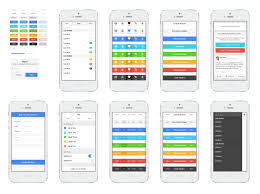
\includegraphics[width=8cm, height=8cm]{Images/ionicUI.jpg},
\caption{Ionic}
\label{ionicUI}
\end{figure} 

\subsection{Angular}
Angular represents a framework from Google to create client applications. First, it is aimed at developing SPA-solutions single-page applications. In this respect, Angular is the successor of another AngularJS framework. At the same time, Angular is not a new version of AngularJS, but a fundamentally new framework.

Angular 5 provides functionality such as two-way binding, which allows you to dynamically change data in one space, including templates, routing, and so on.

One of the key features of Angular is that it uses Typescript as its programming language. But we are not limited to Typescript. If you want, you can write the Corner applications with languages such as Dart or JavaScript. However, Typescript is still the main language for Angular.

One of the key elements of the application are the components. The component controls the display of the presentation on the screen. \cite{angular} \\

\begin{figure}[ht]
\renewcommand\thefigure{4.2}
\centering
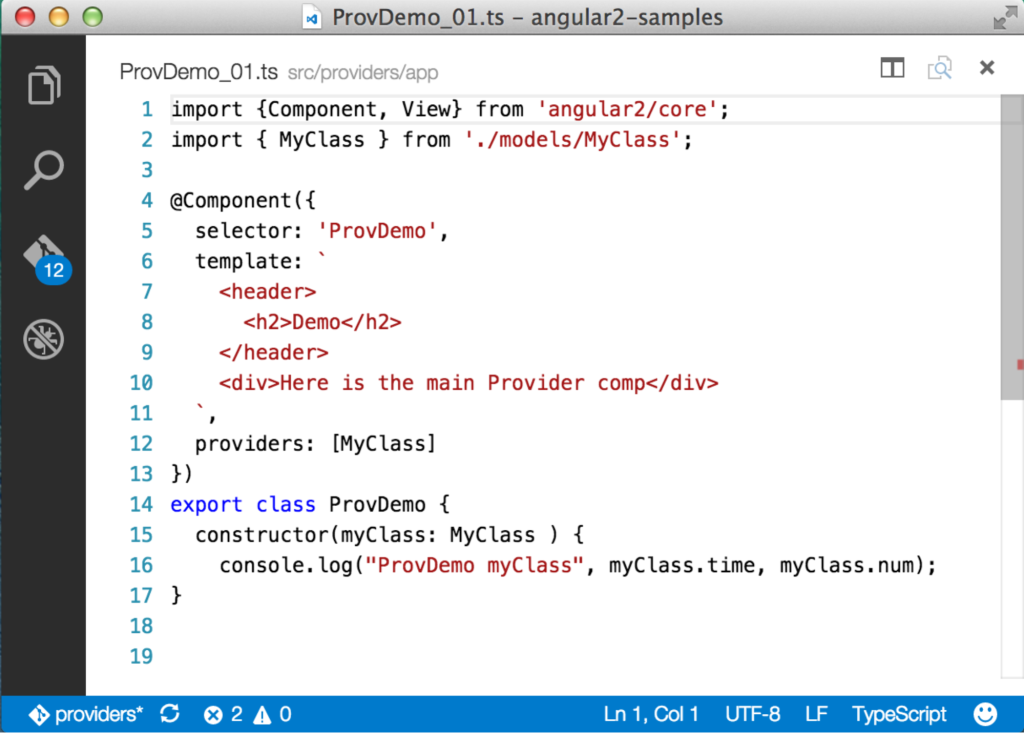
\includegraphics[width=8cm, height=8cm]{Images/angular.png},
\caption{Angular-Component-Example}
\label{angular}
\end{figure} 

For a class to be used in other modules, it is defined with the export keyword. In the same class, only one variable is defined, which stores a string as a value. To create a component, you need to import the @Component decorator
function from the @angular/core library. The decorator @Component allows us to identify the class as a component.

If we did not apply the decorator @Component to the AppComponent class, the AppComponent class would not be considered a component.
The decorator @Component takes as an argument the object with a configuration that specifies the framework, how to work with the component and its representation.

\section{Languages}
\subsection{Typescript}
Typescript is backwards compatible and compiled in JavaScript. In fact, after compilation, the program written using Typescript can be executed in any modern browser or used in conjunction with the server platform NodeJS.
The code of the compiler that translates Typescript in JavaScript is distributed under the Apache license.

Typescript differs from JavaScript in the ability to explicitly enforce static types, support the use of classes, as in traditional object-oriented languages, and support for connecting modules, which is designed to improve the development speed, facilitate readability, refactoring and reuse of code, search for errors at the stage of development and compilation. Typescript also accelerates the execution of programs. \cite{TS}

\subsubsection{Services instead of Factories}
When Angular switched to typescript from JavaScript it moved away from using factories to using services. 

To implement the service, we pre-announce the interface for the service that we are exporting. Then we create a class for the service that implements the service interface. And then we call the Angular method to add the service. \cite{TS}

\begin{figure}[ht]
\renewcommand\thefigure{4.3}
\centering
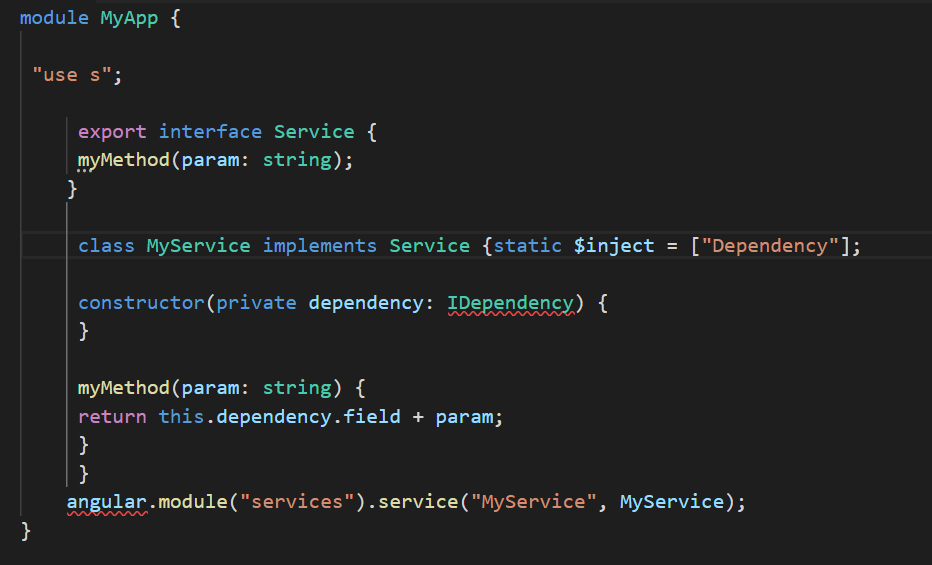
\includegraphics[width=12cm, height=7cm]{Images/TS.png},
\caption{TS-Example}
\label{TS}
\end{figure} 

Above is an example of a snippet of code I wrote to show how the services can be used in our Typescript Application.
The constructor parameters declared with private or public modifiers become class fields and get values corresponding to the values of the constructor parameters. If we look at the following link we can understand clearly why this is a much better method to use than Factories \cite{factory}

\subsection{HTML}
HTML is a hypertext mark-up language, which is used to create documents on the Internet (web pages). The web page is created using HTML that contains all the necessary elements. On the HTML page, you can place a simple text, highlight it in bold or italic, insert a link, a table, a numbered or unnumbered list, pictures, divide the text into paragraphs and sections and specify headings for sections. Also, on the HTML page, you can insert a form with text fields, buttons, select options from the list, check-boxes and radio elements. In HTML5, you can embed video and audio files in a page,
draw with canvas, make simple animations with new tags. Below is a quick snippet of a 'Hello World' HTML example page.
\cite{html}

\begin{figure}[ht]
\renewcommand\thefigure{4.4}
\centering
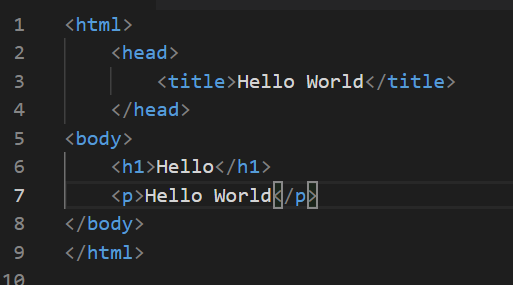
\includegraphics[width=10cm, height=5cm]{Images/html.png},
\caption{HTML-Example}
\label{html}
\end{figure} 
 
\subsection{SCSS}
SCSS(Sassy Cascading Style Sheets) is a super set of css. So first of all I'll explain what css is as it covers a lot of what Sccss does. CSS - 'cascading style sheets'. 
In fact, they serve to separate the page structure and its content from its appearance. If the page is completely written in HTML, then each element of the code determines not only the content element of the page but also its way of displaying. For example, not only that there is a text ”Hello” in such and such a place, but also that this text is highlighted in bold and red. With the use of CSS code, everything happens a little differently. 
With the help of HTML, only the order of the content elements of the page and their classes are described. The corresponding classes are written in the CSS file. Each of them is assigned a set of properties. Then when we assign a class to an HTML element, then all the properties of this class are applied to it. This greatly reduces the repetition of code. However, when sites have many pages, you can not do without CSS. \cite{css} \\

Having covered CSS we now have the basics of SCSS.SCSS and css are the exact same whereas we just regard SCSS as a higher class of CSS styling, SCSS offers a much more detailed design for our Application also. The only commanding difference between the two is that SCSS allows the use of declaring specific variables which you can use throughout the SCSS file. This saves the user a great deal of time and also allows for more uniform results on the HTML page. I will provide examples of both CSS and SCSS below and the difference can clearly be seen between the two.

\begin{figure}[ht]
\renewcommand\thefigure{4.5}
\centering
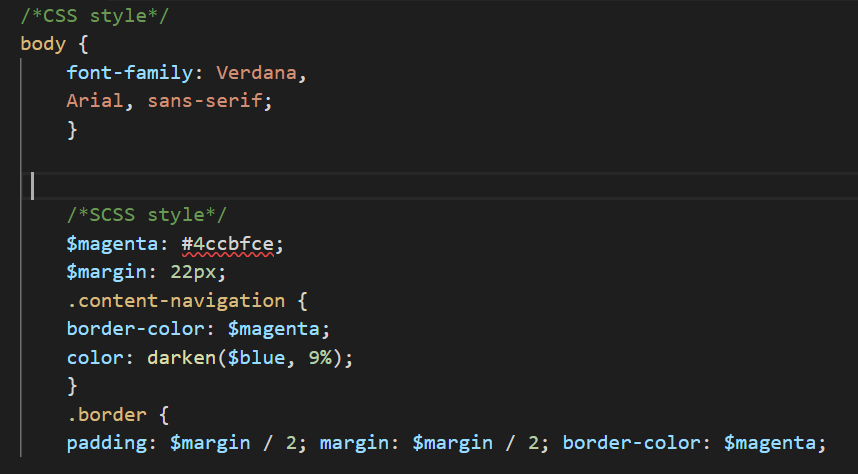
\includegraphics[width=10cm, height=5cm]{Images/scss.png},
\caption{css/scss-Example}
\label{scss}
\end{figure}

\subsection{JavaScript}
JavaScript is a scripting or programming language that allows you to implement complex things on web pages — every time a web page does more than just sit there and display static information for you to look at — displaying timely content updates, interactive maps, animated 2D/3D graphics, scrolling video jukeboxes, etc. you can bet that JavaScript is probably involved. It is the third layer of the layer cake of standard web technologies, two of which (HTML and CSS) we have covered in much more detail in other parts of the Learning Area. \cite{js}

As of today JavaScript is currently working on JavaScript2.

\subsection{LaTeX}
LaTeX is a typing system used throughout industries. It works on a scripting programming language. LaTeX is not as simple and understandable as the likes of Microsoft Word but it is a much better resource than Microsoft Word. LaTeX is a de facto understand and has been for the last number of years for the writing of papers such as articles, reports and in our case a Dissertation. It can be confusing at the start to understand how it works and may confuse a lot of people but it is the best tool for writing up these type of files. LaTeX allows the writer to just concentrate on the actual writing of the paper rather than worry about how the layout will look and where to position certain items as LaTeX uses its scripting language to do so. \cite{latex}

\begin{figure}[ht]
\renewcommand\thefigure{4.6}
\centering
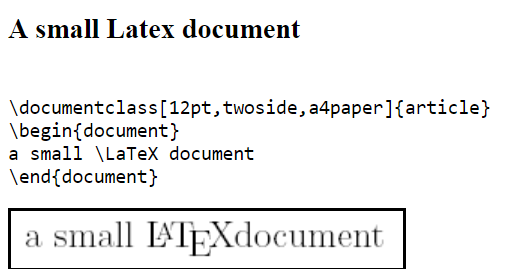
\includegraphics[width=10cm, height=5cm]{Images/latex.png},
\caption{Small LaTeX Document}
\label{latex}
\end{figure}

\section{Software and tools used}

\subsection{Visual Studio Code}
Microsoft has released many development tools. But probably the best they have ever released would have to be Visual Studio Code working on three platforms, Linux, OS X and Windows. Without throwing all the functions of a mature Visual Studio IDE. Microsoft decided to rethink the approach on which the main toolkit of the programmer is built and started with the most important - the code editor. Visual Studio Code is an editor, but it has IDE functions that rely on extensions. 

Now with Visual Studio Code is possible to use different languages such as JavaScript, Typescript, C sharp, and so on. Also, you can use Visual Studio to create ASP.NET 5 or NodeJS web projects, work with package managers npm and even carry out debugging. An excellent intellisense, support for code snippets, refactoring, navigation, multi-windowing, git support and much more. In some ways, Visual Studio Code even more convenient than the full version of Visual Studio and much lighter for the hardware requirements.

We both have experience of using Visual Studio Code in the past along with using a number of extensions so decided it best suited our approach.

\subsubsection{Visual Studio Code extensions}
Without the Visual Studio Code extensions, it's only suitable for simple editing of files, for proper work you will need the accompanying tools that depend on your goals and tasks:
\cite{vsDocs}

\begin{itemize}
\item git - version control system

\item NodeJS (includes NPM) - a platform for creating scalable network applications

\item Express - a framework for Node applications

\item generator-aspnet - yeoman generator for ASP.NET 5 applications, run npm install -g generator-aspnet for installation

\item gulp - a toolkit for creating and performing tasks associated with the assembly of project tasks

\item Typescript - Typescript language, adds modularity, classes and other nice things into your JavaScript code

\item Typescript definition manager - Typescript definitions for popular JavaScript libraries, include support for IntelliSense in the VS Code 

\end{itemize}

\subsubsection{Command Palette}
The most important tool for interacting with the editor in VS Code is the command palette. You can call it via the keyboard, by pressing the combination Ctrl + Shift + P. A lot of commands listed in the palette are also attached to the keys. These is very helpful for using in an ionic project where some files can be hard to find by manually searching through folders. \cite{vsTips}

\subsubsection{Auto-save}
By default, VS Code works in the explicit save mode, which you can perform by pressing the Ctrl + S combination. This mode is compatible with most status monitoring tools. You can turn on the auto-save mode by pressing Ctrl + Shift + P and type auto. \cite{vsTips}

\subsubsection{IntelliSence Tips}
Wherever you are in your code, clicking on Ctrl + Space will display the IntelliSence prompt. When typing the code, the editor will show it automatically. \cite{vsTips}

\subsection{GitHub}
GitHub is a hosting service which allows users to host, share and collaborate on projects together. It can be used freely for Open Source projects. Projects hosted on GitHub are called repositories. It is here users can view their projects, pull down a version of this project to their device or add to the project depending if you are either the owner of repository or a collaborator on the repository.

Collaborating on projects especially coding projects can get very complicated as others peoples work can conflict and disrupt the process. Luckily GitHub takes care of this with its distributed version control. Allowing the user to revert back to changes at any stage of the project, branch to different work trees and also merges branches back together.

In addition to being just a hosting project, GitHub is also a great social networking site for developers and programmers. It allows users to follow each other, subscribes to project updates, like them, giving them an assessment, etc. These functions allow users to receive updates for projects in which they are interested, or stay in touch with colleagues and employees. GitHub has been described as a portfolio for programmers work and many employers would ask potential employees for their GitHub profile link to review their work.

GitHub is not only used for programming and software development. It is also used by many other types of projects. For example, open source tutorials, documentation projects, training resources and other projects in which users can work together. \cite{github}

A few simple git commands that are most commonly used when working on git projects would be:

\begin{itemize}

    \item git add . \\
    Adds all files that are not already pushed to your GitHub repository.
    
    \item git commit -m "Commit message" \\
    To commit changes and give your commit a message 'Commit message'
    
    \item git push  \\
    A simple 'push' to your repository on GitHub 
\end{itemize}


\subsection{Overleaf}
Overleaf is an online real time LaTeX editor which allows us to write our text documents on a site without needing an special software installed on our machines. 

We both decided to use this platform as we used in earlier in the year when writing up  our literature review assignment which also required us to use LaTeX. 

Overleaf offers a lot of features that will work perfect for our project. We can work collaboratively on the document at anytime, it offers the choice to link the .TeX files straight to our GitHub repository if needed but we opted to just manually download our PDF version and add it to our ionic project folder for now until we have completed the documentation.

Overleaf has a history section which allows us to look back on all the work carried out in the document, pin-point it to a date and see which one of us was working on the document at that time. It is also extremely convenient if any mistake were to happen, which is most likely to happen when collaborating on a project, we can use this section to go back a step or two and recover our work and fix any of the errors.

\chapter{System Design}
In this section, we will cover the overall design and architecture of our Application. We will do this through code snippets and visual aids to help you get an understanding of the Application design. The System Design chapter will be broken up into four parts. Data Tier represented by our Databases CouchDB, Mongo DB and Firebase Authentication, Logic Tier represented by NodeJS server, Presentation Tier which will be represented by Ionic 3 App and our Application deployment. The figure in 5.1 shows the overview of our Architecture.

\begin{figure}[ht]
\renewcommand\thefigure{5.1}
\centering
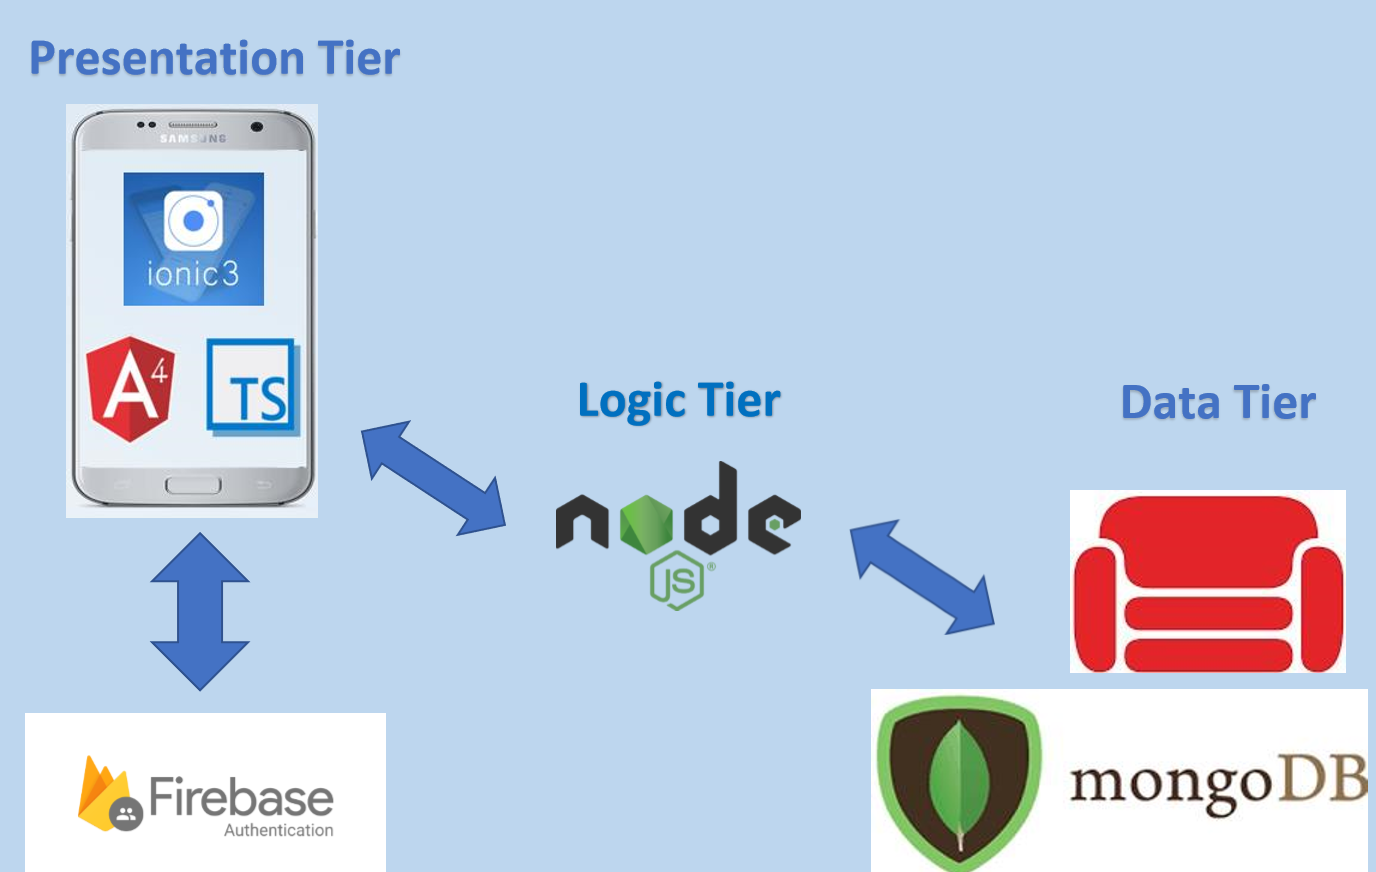
\includegraphics[width=13cm,height=7cm]{Images/architecture.png},
\caption{Architecture}
\label{Architecture}
\end{figure}

\section{Data Tier}
The data tier represents the overall stored data and gives the ability to store, access, update and delete certain data. For our application we have three databases that we are using. One for storing our users and the other two for storing different data in the Application at different sections.

\subsection{Firebase Authentication}
We chose Firebase to handle our user accounts as it was established in the Ionic community for being a good database for login and registration functionality. We chose to use this free Authentication API service as it offered ready made functionality such as password reset, email and password authentication and gave us the options to add additional login options such as Google login or Facebook login etc. We both have experience of using this feature so found it would best suit us towards the making of the app.

\subsection{CouchDB}
We decided to use CouchDB for storing the data that a user can add in our Medicine section. We found it very simple to use as we can visually see our data being added on a localhost which is where we must call from in our app to create the database. The stored data can be viewed in JSON format which is easily read for us in order to test whether it is interacting with our app. As happens with any development stage some changes may need to take place, we considered this when choosing our databases, CouchDB makes it very simple to change what is being stored to the database allowing us to make any quick changes to how are app looks.

\subsection{MongoDB}
We chose Mongo DB to store our users tagging and AI information, also our users forum messages and adding images to the forum as it offers a lot of flexibility. As with CouchDB giving us the functionality to change how our database looks we can also do the same for mongo which is very helpful when wanted to make big changes to our application. Mongo allows you to download and host your own Mongo DB server for free. This download comes with its own terminal which you can use to query your database which was very effective tool during development.

\subsection{Collections}
Our MongoDB will be structured into different collections:

\begin{itemize}
    \item Taggings - Store tagging models
    \item AIs - Store AI models
\end{itemize}

Below is a small example of our tagging property layout:
    
\begin{figure}[ht]
\renewcommand\thefigure{5.2}
\centering
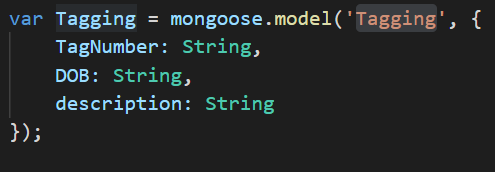
\includegraphics[width=10cm,height=4cm]{Images/modelJSON.png},
\caption{JSON Example}
\label{json}
\end{figure}


\section{Logic Tier}
Logic tier refers to your apps business logic. It his here we program your applications ability to manipulate data. These include creation, storing , updating and deletion of Data. To handle our business logic we use NodeJS. NodeJS was the obvious choice for our three tier architecture not only does it link up well with our MongoDB but also is easily integrated with our Ionic three presentation tier. NodeJS with its light-weight nature and its scalability due to its non-blocking I/O calls allowing tens of thousands of concurrent connections made it more than capable for our application. Using Javascript for our logic tier and using type-script for our providers in our presentation tier made it really easy to transition between the two because of their similarities.

\subsection{Connection to Data Tiers}
For creating the connection between the Data Tier and the Logic Tier we used Mongoose. Mongoose is a JavaScript library which allows us to define a schema with strongly typed data. Mongoose then allows you create models which map to a MongoDB Document via the Models schema definition. \cite{mongoose}
\\
Not only does Mongoose allow you to define strong data models and the ability to manipulate them before saving, it also offers functions to create an easy connection to your database and to validate,save,delete and query your data. Below you can see an example of this from our Farming App: 

\begin{figure}[ht]
\renewcommand\thefigure{5.3}
\centering
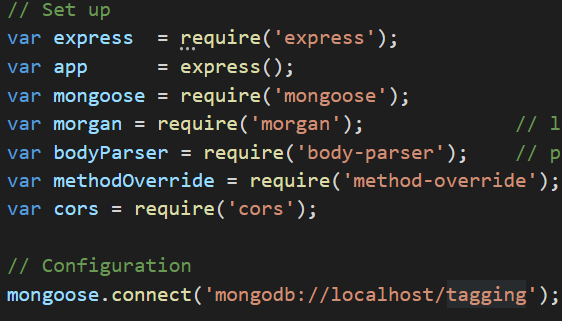
\includegraphics[width=10.5cm,height=6cm]{Images/setup.png},
\caption{Server Example}
\label{setup}
\end{figure}

Shown in figure 5.2 we can see our tagging data model and how we are declaring each data type.

\subsection{Connecting to Presentation Tier}
We are looking at the logic tier at the moment so I will quickly look at how we are connecting from our logic tier to our presentation Tier. In the Logic tier we have configured our farm server to run on port 8080. It is on this port where our servers will send and receive traffic to our presentation layer. Using our IP address, port number and routing address, the presentation tier will be able to send http requests to our server. Depending on the routing address provided will determine what action the server will take on our data tier.
\\

\newpage

\subsection{Routing and Accessing data}
Here we will show some of our routing and mongoose functions which allow to us to query our data tier MongoDB and CouchDB. 

\subsubsection{MongoDB}
First we will go through how we are using MongoDb in our application and later on we will discuss our CouchDb database.\\

But, First up we will see our HTTP get request being performed in our taggings collection. We access this function by using its routing address which can be seen in the below figure.

\begin{figure}[ht]
\renewcommand\thefigure{5.4}
\centering
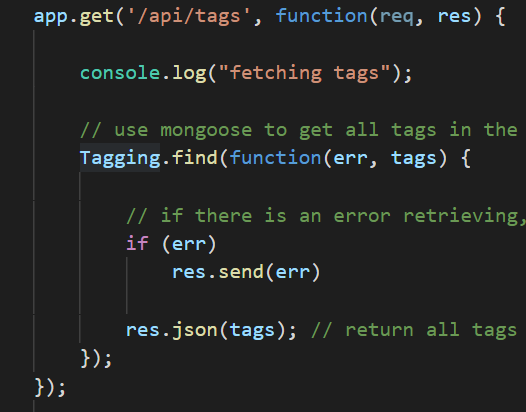
\includegraphics[width=11cm,height=5.5cm]{Images/get.png},
\caption{Get Request}
\label{get}
\end{figure}

This function will return an array of room objects from the database and send them to our Ionic application in JSON format.
\\


Our next function will be the POST request on the taggings collection. We access this function by using its routing address which can be seen down below.\\

\begin{minted}{js}
app.post('/api/tags', function(req, res) {

            console.log("creating tag");
    
            Tagging.create({
                DOB : req.body.DOB,
                description : req.body.description,
                TagNumber: req.body.TagNumber,
                done : false
            }, function(err, tag) {
                if (err)
                    res.send(err);
    
                Tagging.find(function(err, tags) {
                    if (err)
                        res.send(err)
                    res.json(tags);
                });
            });
    
        });
\end{minted}



As you can see above we create a Property object with the data received from body of our http request and post to our properties collection. After we do this we then perform a get request and return the new refreshed array of property objects to our Ionic application.\\


So far we have shown how to send and retrieve data to our MongoDB database.\\


Next I will explain how we can delete data from our database. We also have the option to update the data in our database but for the mean-time we have opted against using this as the data that a user is storing cannot be updated to allow them to alter their data.\\

Below I will show how we use the delete function in our taggings collection.

\begin{minted}{js}
    app.delete('/api/tags/:tag_id', function(req, res) {
        Tagging.remove({
            _id : req.params.tag_id
        }, function(err, tag) {

        });
    });
\end{minted}

\newpage

The same process is required for our MongoDb database for AI as above. We will use the same HTTP requests just create a new database with a new collection and will be routing to this collection where we can store our data.\\

\subsubsection{CouchDB}
CouchDB is fairly similar to MongoDB when it comes to storing data to a database where it also uses the HTTP request methods. There is no need to setup a seperate server folder for Couch however, as all we must do is import PouchDB to our ionic project and make a call using PouchDB to where we created.

In the figure below I will show how this is done:

\begin{figure}[ht]
\renewcommand\thefigure{5.5}
\centering
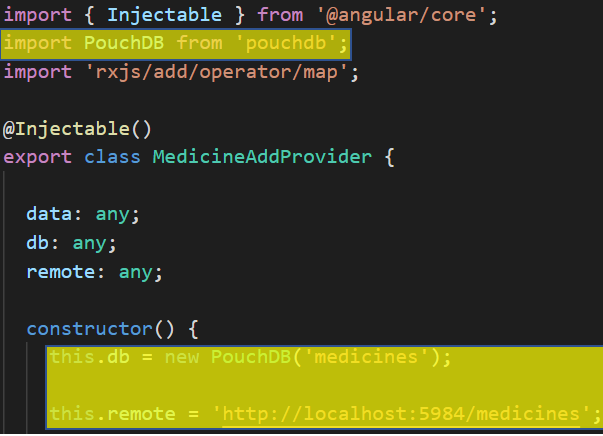
\includegraphics[width=11cm,height=5cm]{Images/pouch.png},
\caption{CouchDB}
\label{couch}
\end{figure}

In order to retrieve our data from the database we made a function 'getMedicine' which will return all our medicine data stored on CouchDb. We needed to create variables like 'data,db,remote' in order to carry this out.\\


We then used a 'handleChange' function which gives us the operations to delete, update and add our data to the database.

To add to the database or to delete we simply used the two following functions to do so:\\
\begin{minted}{js}
    createMedicine(medicine){
    this.db.post(medicine);
    }
    

    deleteMedicine(medicine){
    this.db.remove(medicine);
    }
\end{minted}

\newline

We simply then just call these two functions in our page for medicine in order to 'POST' to our database or 'delete' from it. Note that CouchDb uses the 'remove' keyword and not the DELETE HTTP request.\\

We also use our 'getMedicine' function in the same page in order to retrieve the data from our database and have it displayed on the page.\\

An extra function that we have added with CouchDB is a search function. This is done by creating 'Pipes' which allows us to add a search bar to the top of our page and it will search for 'terms' of the data stored. The user will simply begin to type what they are looking for and the page will start filtering through the list by letters and will only show what the user has searched for. We will discuss pipes down below.

\section{Presentation Tier}
In the Presentation Tier section will be looking at five areas. We will look at how our Ionic 3 app is structured, we will look at how our providers are interacting with out NodeJS server and with our Data Tier databases, we will have a quick look through each of our Applications pages showing how they look and also some functionality, we will quickly discuss the use of Pipes in our application, and finally how we used SCSS in designing our applications style.

\subsection{Ionic 3 App Structure}
First of all we have our Ionic 3 App structure which can be seen the below figure.


We will give a brief explanation to each folder that can be seen in figure 5.6:

\begin{itemize}
    \item Node-Modules - Here contains the packages required to run and develop this ionic App
    \item src - is the folder where we will do most of our coding for our Ionic 3 app. In here we will be using SCSS, typescript, angularjs and javascript.
    \item WWW - is where our index.html lies and is the root component where the app will load
\end{itemize}
%% make edits here once app is finished
\begin{figure}[ht]
\renewcommand\thefigure{5.6}
\centering
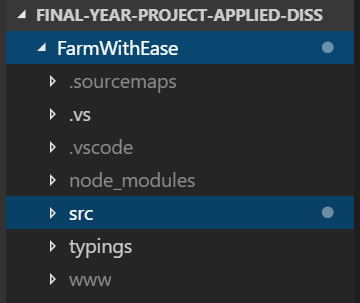
\includegraphics[width=8cm,height=5cm]{Images/app.png},
\caption{App Structure}
\label{app}
\end{figure}

In the src folder Ionic 3 have structured our components into well thought out Folders as seen in figure 5.7 below.

\begin{itemize}
    \item App – This is where we set up the base of our app. In here we provide access to components (such as other pages, providers etc) for various pages in our App as well as creating the App shell. For example whether our App will be a side Menu or tab style Application structure.
    \item Assets – Folder containing any images/icons.
    \item Models - In here we create our object models. For example we have our User Model here which is made up of a String Email and a String Password.
    \item Pages – This is where the majority of our presentation tier code goes. Here is where we go through our pages design and how they will function for us. We will be going into each page in more detail below.
    \item Pipes – In our pipes folder we link up with our list arrays to perform a search in our medicine and AI section where we can search for a specific name of a medicine or whether or not a cow is 'In Calf' or not.
    \item Providers – This is where we link our Application to our Logic Tier Servers. We have three providers that is looking after our tagging, AI and medicine sections. In the next section we will show you how we accomplish this.
    \item Theme– This allows us to set the overall design and look of our app through global SCSS.
    %\item Validators – In here we provide functions to validate whether users input was correct. I.e valid email address.
\end{itemize}

\subsection{Providers}
The providers give our application to our data tier through our servers. It is here where we apply the logic and perform HTTP requests to our Node servers to either return, create or delete data from a server. It is in this folder where we make the connection from our Ionic Application to our specific data base on the server.

\subsection{Pages}
Ionic 3 pages are broken up into four parts:

\begin{figure}[ht]
\renewcommand\thefigure{5.8}
\centering
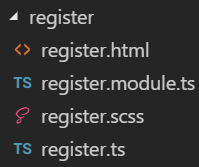
\includegraphics[width=6cm,height=4.5cm]{Images/pages.png},
\caption{Pages layout}
\label{pages}
\end{figure}

In fig 5.8 we can see how our register page is laid out with 4 different parts.

\begin{itemize}
    \item \textbf{register.html:} HTML file which creates the overall layout of the page. Adding forms, lists, buttons and images where needed. With the Ionic framework we can use angular directives on html elements such as buttons which offers us greater functionality and design. For Example:
    \begin{minted}{html}
        <button>Hello World</button>
    \end{minted}
    \item \textbf{register.module.ts:} This page is auto generated when generating the page. It is seen as the deep thinking part of our page. We do no actual code changes here to design our page.
    \item \textbf{register.scss:} The SCSS design of the page.
    \item \textbf{register.ts:} TypeScript file which handles the logical function of the page. Here we code our individual functions and bring in our imports needed for functionality.
\end{itemize}

We will now go through our Applications pages below.

\subsubsection{Login Page}
% edit here if google login added

This page will be the first page greeted by the user when opening the app. It is here where they can login to their account(if one exists) with an email address and password. When entering the email and password, validation is performed to ensure that the email is the right format, the password contains the right characters and length and all field are filled. Firebase Authentication is used here which it will query our Firebase API to check if they user exists in our Firebase Database.

If the user is logged-in successfully, the API will return the users details to the screen, a session key to grant access to the apps features and will allow our user to be navigated to the Home Page of our App. If the user is new to our they can click on our Register button which navigate them to our register page where they can enter their details to be given an account.

If the user forgets their password, a 'forgot password' button is available on this page also which when clicked on by the user will bring them to a forgot password page. 

\begin{figure}[ht]
\renewcommand\thefigure{5.9}
\centering
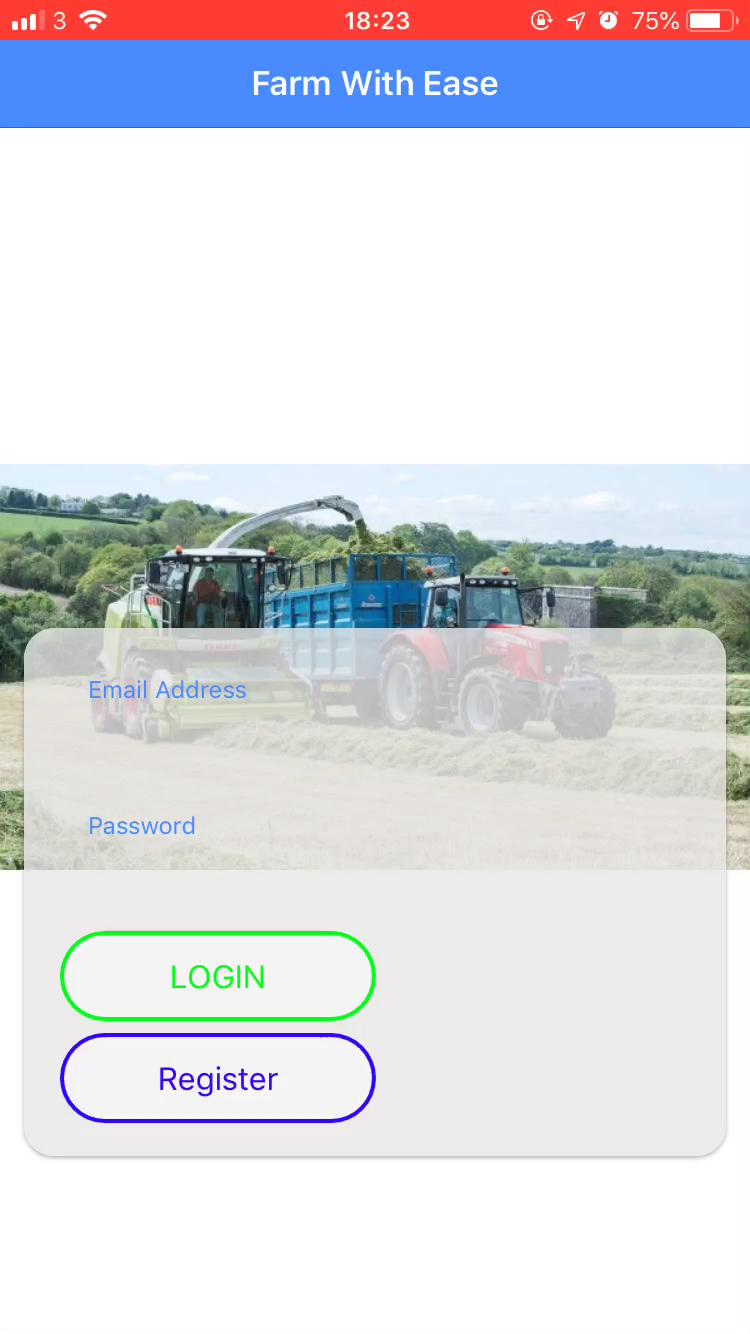
\includegraphics[width=4.5cm,height=7cm]{Images/loginPage.jpg},
\caption{Login Page}
\label{login}
\end{figure}

\subsubsection{Register Page}
When the user enters the register page they will be prompted to enter an email address and password in order to register their account. The same validation progress is performed here as with the login page as the email and password fields. When the user clicks 'Register', our Firebase API will store the user details, will return a session key in order to grant the user access to our App. Upon completion of registration the user will be navigated to the home page.

\begin{figure}[ht]
\renewcommand\thefigure{5.10}
\centering
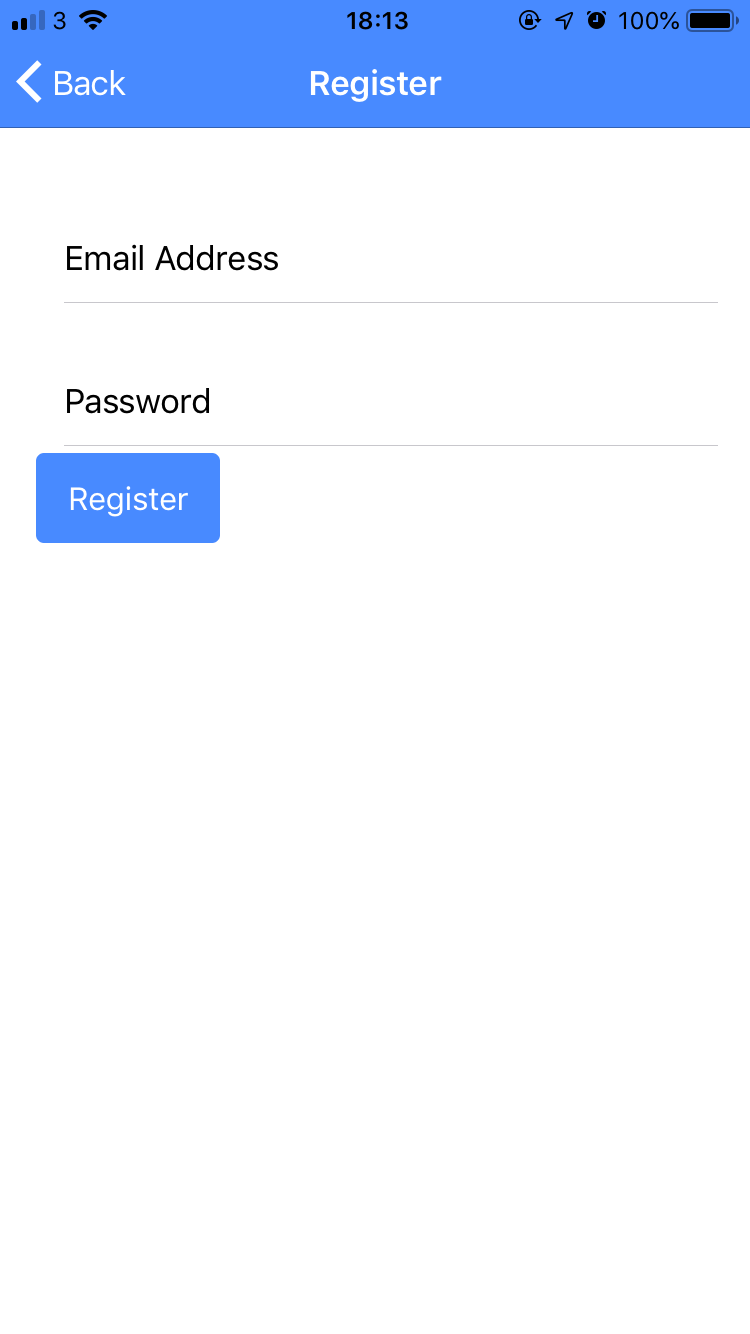
\includegraphics[width=4.5cm,height=7cm]{Images/registerpage.jpg},
\caption{Register Page}
\label{register}
\end{figure}

\subsubsection{Forgot Password Page}
Here the user will be asked to enter their email address and to tap the reset button. If the email is a registered email address the user will be asked to check their email account and follow the instruction to reset their password upon receiving an email from FarWithEase.

\subsubsection{Side Menu}
Our side menu will give the user the navigation options throughout the App. The menu is available once a user is logged in. Once logged in users can navigate freely throughout the App by using all the options available in the side menu.

If a user decides they are finished using the App and wish to logout, we have a logout button which will logout the user and return them to the login page.

\begin{figure}[ht]
\renewcommand\thefigure{5.11}
\centering
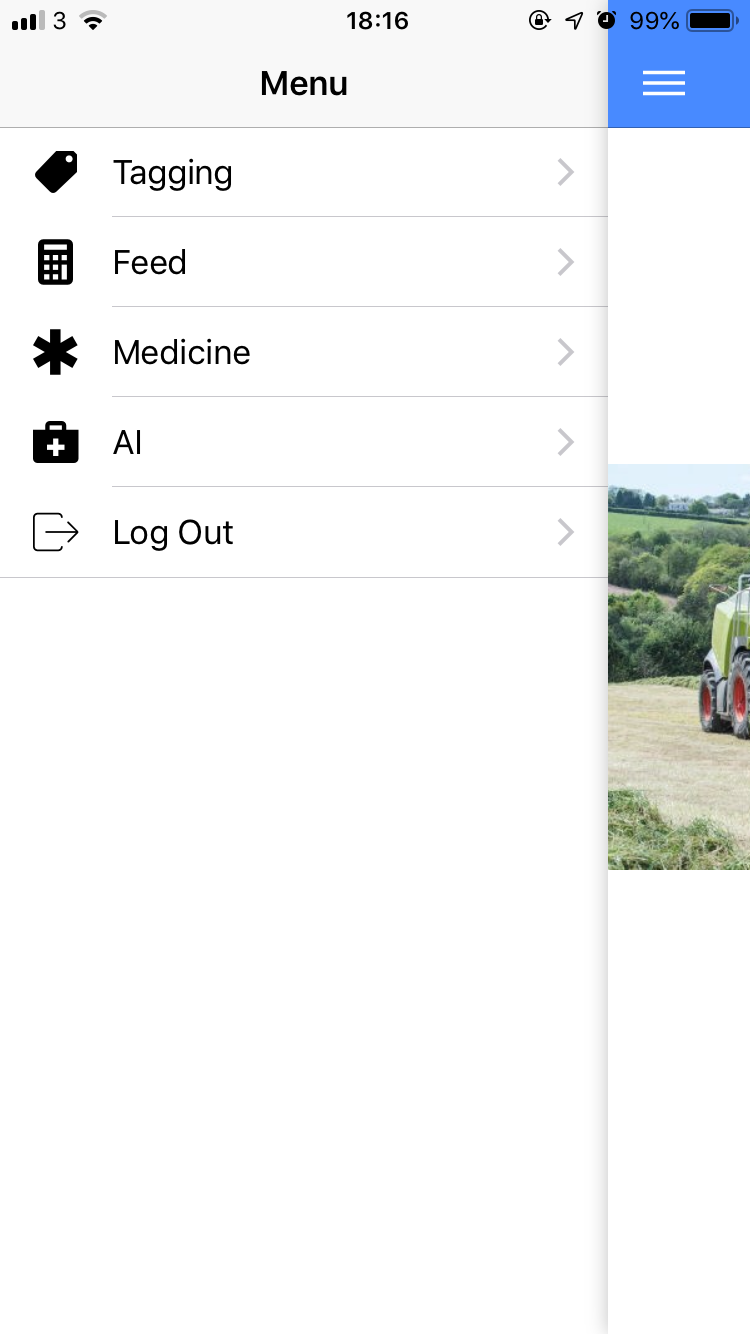
\includegraphics[width=4.5cm,height=7cm]{Images/sideMenu.jpg},
\caption{Side Menu}
\label{menu}
\end{figure}

%\subsubsection{Home Page}

\newpage
\subsubsection{Tagging Page}
Our tagging page is where our user can add all their livestock that are tagged to keep them in their records. The user can tap on the add icon on the top left on the page which will pop up a modal where the user can input their data(we will discuss the modals later). Once the data is entered and saved it will be displayed as a list in the tagging page. If the user wishes to the delete the data they can swipe left to view a trash can which will delete the data from the list and also from the database where it is saved.

At the top of this page we have also added a search bar for our users to search their information by Breed.

\subsubsection{Feed Page}
Our feed page is very different to our other pages where it is here where specific calculations can be carried out by a user in regards to silage quantity, pit sizes and how much bales of silage they need, have or will be left with in their own specific scenario. 

\subsubsection{Medicine Page}
For our medicine page we have designed it so that the user can easily input data for what medicines they have used on a certain animal. The add icon will be displayed in the top right corner and will pop up a small input box with different information that a user can add to the list and database. The user will also have the option to delete this information later on if they wish so. We decided that the update function should not be used here as it is not the right thing for a farmer to be editing what medicines they are using on the farm.

As like in our Tagging page we have a search bar here also so we can search for our medicine names.

\subsubsection{AI Page}
On the AI page we decided to make we are giving the users the feature to keep record of all the calving and births that is happening on their farm. The farmer can enter the cows tag number, how many weeks she has been in calf, and also whether she is in calf or not. This section can be used as a way for a farmer to keep a total record of their cattle and then to also track any pregnancies along the way.

As above our search bar is also in this page where a user can filter their information by whether a cow is in calf or not.

\subsubsection{Add Pages for Tagging and AI}
You can see the layout for our search pages from figure 5.12  below. These pages are presented to the user when the click on the add icon on the relative pages for tagging and AI. The user can fill out the form on these pages as appropriate to their needs. Once all areas are filled out the user can click the save button which will return them to the previous screen but this time their entered information will be displayed on the list will all relative fields entered displaying. 

\subsubsection{Add to Medicine}
This add section is different to above as it is not an actual separate page. For this section we opted to use a prompt function just to simply demonstrate the different ways how adding items to a page could be done. It works in the exact same way as the pages for tagging and AI where we have a form that needs to be filled out, at the bottom we have a cancel and save button. Cancel will just exit the procedure and return to the page, clicking save will save the data entered and return it to the medicine page where it will be visible to our users.

\subsubsection{Medicine Scanner}
This page is where a user will locate a a bar cod scanner which they can use if they wish to scan a medicine bottle they are using on an animal and it will return data back to them giving information about that certain medicine being used.

%\subsubsection{Search Page}

%\subsection{Styling}

\subsection{Deployment/Hosting}
For now we have decided to host our project locally on our own machines for testing purposes.

We first must run our MongoDB which is done by opening a CMD prompt and then cd to the location of our bin folder.
\begin{minted}[tabsize=2,breaklines]{bash}
C:\Program Files\MongoDB\Server\4.0\bin>mongod
\end{minted}

Once this is running we then must go on to run our server.js file in our folder. We do this again by opening the node CMD prompt and cd to our server file location.
\begin{minted}[tabsize=2,breaklines]{bash}
C:\Users\Gary Mannion\Desktop\Final-Year-Project-Applied-Diss\server>node server.js
\end{minted}

Once all these steps are done we can then cd to our Ionic app location and start it.
\begin{minted}[tabsize=2,breaklines]{bash}
C:\Users\Gary Mannion\Desktop\Final-Year-Project-Applied-Diss\FarmWithEase>ionic serve
\end{minted}

Once all the above has been completed the app should be running as intended to.

\chapter{System Evaluation}
In this chapter we aim to evaluate our system in the following areas:
\begin{itemize}
    \item Robustness
    \item Testing
    \item Limitations
    \item Results V Objectives
\end{itemize}

\section{Robustness}

\section{Testing}
Through continuous white box testing and regular black box testing we believe our App has reached the expectations we set out at the start of our project. In order to achieve these expectation we carried out testing using our white box testing in the following ways:
\begin{enumerate}
    \item Ionic Serve
    \item Device Testing
\end{enumerate}

\subsection{Ionic Serve}
We used this method of testing in our browser as it could be used alongside the development of the App while were carrying work. We simply just cd to the root of the Ionic App folder and run the following:
\begin{minted}{bash}
ionic serve
\end{minted}

This testing method was very helpful in the development of the app as it provides a live-reload server. This meaning whenever we made a change in any part of our code(HTML, TypeScript or SCSS) the changes would automatically reload in the browser.
\\
There is also the option of running the command:
\begin{minted}{bash}
ionic serve --lab
\end{minted}

This would show us a preview of how each change would appear in Android, IOS and Windows platforms.

\subsection{Device Testing}
We opted to use the Ionic DevApp Application from the iOS store for testing on iOS devices. This was helpful for getting an idea of the app was functioning on the iOS devices but it needed to be connected to the same network as the laptop it was connected with so was not the best option.\\

\noindent
Instead we decided to build an Adnroid APK file which we could then install on an Android device and do some better testing from there.

\section{Limitations}

\section{Results V Objectives}

\chapter{Conclusion}

\section{Future Development}

\chapter{Appendix}

\textbf{Project Source Code Link:} \\
%\item \href{https://github.com/Gazza1996/Final-Year-Project-Applied-Diss}{https://github.com/Gazza1996/Final-Year-Project-Applied-Diss} 

\bibliographystyle{ieeetr}
\bibliography{Bibliography}

\nocite{*}


\end{document}